\section{Theory and Algorithms}
\label{sec:theory}

Let us first consider a scenario where the GBR $z\xrightarrow{G}_+r$
on circuits under RTTO can result in a size explosion (expression
swell) problem in an explicit representation. We also show on the
other hand that an implicit set representation (ZBDD) overcomes 
this size explosion. 

\begin{figure}[hbt]
\centering
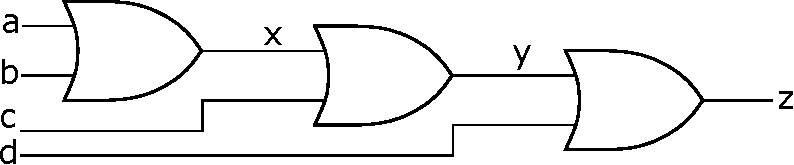
\includegraphics[scale=0.40]{Preliminaries-Theory/Chain_Or_Gates.pdf}
\caption{A chain of OR gates.}
\label{ChainOrGate}
\end{figure}


\begin{figure*}[hbt]
\centering
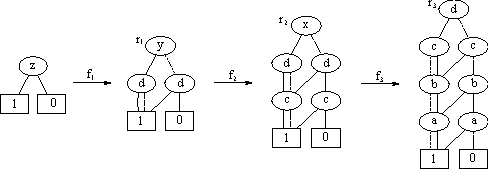
\includegraphics[scale=1.4]{./Preliminaries-Theory/red_steps.pdf}
\caption{Reduction of output of the circuit in Fig. \ref{ChainOrGate} by $f_1,f_2,f_3$.}
\label{red_steps}
\end{figure*}

Consider the circuit shown in Fig. \ref{ChainOrGate} consisting of a
chain of OR gates. Impose RTTO: i.e. {\it lex} term order with
variable ordering as, $z>y>x>d>c>b>a$. The Boolean polynomials for the
circuit are: 
\begin{align}
f_1 = z + y d + y +d;\\ 
f_2 = y + x c + x +c; \\
f_3 = x + b a + b +a;
\end{align}

Under RTTO, the set $G = \{f_1, f_2, f_3\}$ forms a GB. To derive a
canonical representation of the function, we have to reduce the
output $z\xrightarrow{G}_+r$. A classical symbolic algebra
reduction using an explicit representation is carried out as follows: 

\begin{enumerate}
\item { $z \xrightarrow{f_1} y d +y +d$}
\item { $y d +y +d \xrightarrow{f_2} y + xdc + xd + dc + d \xrightarrow{f_2} xdc + xd + xc + x +dc + d + c$}
\item { $xdc + xd + xc + x +dc + d + c \xrightarrow{f_3} xd + xc + x  +
  dcba  + dcb + dca + dc + d + c \xrightarrow{f_3} xc + x + dcba +dcb
  + dca + dc + dba + db + da + d + c \xrightarrow{f_3} x  +dcba +dcb +
  dca + dc + dba + db + da + d + cba + cb + ca + c \xrightarrow{f_3}
  dcba +dcb + dca + dc + dba + db + da + d + cba + cb + ca + c + ba +
  b +a=r$}
\end{enumerate}


In the first step, $z$ is reduced by $f_1$ just {\it once} as that's the only term. In the
second step, the result of step one is reduced {\it twice} by $f_2$ as
the result has two terms containing variable $y$. Similarly,
{\it four} reductions by $f_3$ are required to 
reduce the result of step two into an expression containing only
primary inputs (which cannot be reduced further). 

{\it Observations:} i) Notice that the size of the final remainder 
corresponds to that of the worst case of a Boolean polynomial:
i.e. $r$ contains $2^n - 1\ (=15)$ monomial terms for $n\ (=4)$ variables. ii)
Classical division algorithms reduce the polynomials 1-step at a time,
where only one monomial is canceled in each step. iii) The number of
1-step reductions can increase exponentially as GBR progresses across
the circuit. 

It is clear that any data-structure that {\it explicitly} represents
each monomial will encounter space and time explosion: this includes
the dense-distributive representation of {\sc singular} computer
algebra tool \cite{DGPS}, or the ones used by
\cite{ciesielski:dac2015,rolf:date16}. The $F_4$-style
polynomial reduction of \cite{lv:tcad2013,pruss:tcad} simulates
division on a matrix $M$ representing the problem. However, each column
of $M$ corresponds to a monomial generated in the division process,
therefore \cite{lv:tcad2013,pruss:tcad} also encounter this size
explosion. 

The use of ZBDDs can help overcome this explosion. Fig. \ref{red_steps} shows
the same reduction of $z$ by $f_1,f_2,f_3$ using ZBDDs (exact
procedure discussed later). The size of the ZBDDs after complete reduction by
$f_1,f_2,f_3$ increases linearly in the number of nodes. Subsequently,
the final remainder has $2\cdot n - 1\ (=7)$ nodes (excluding the
terminal 1 and 0 nodes) for $n\ (=4)$ variables. Notice that while
this controls space explosion, the number of paths (monomials) in the
ZBDD is still exponential in the number of variables. A classical
division algorithm that cancels only one monomial at a time may still
require an exponential number \textcolor{red}{of} iterations. We show how to improve upon
such a situation. 

%\begin{Proposition}
%For the worst case of the Boolean polynomial $F$ with $n$ variables and
%$2^n - 1$ monomials, the ZBDD representation of $F$ consists of
%$2\cdot n -1$ nodes in the graph.
%\end{Proposition}
%\debug{somewhere we need to put the objective}

%{\bf ZBDD Representation:} %% We show how reduction is performed using
%% ZBDDs. 
{\it Problem Setup:} Given a circuit $C$, denote all its {\it nets}
with variables $x_1,\dots,x_n$. Let the total number of gates in the
circuit be $s$; represent each gate of the circuit with a polynomial
$f_i$ in its immediate inputs. Then $F = \{f_1,\dots,f_s\}$ describes
the circuit netlist as a set of Boolean polynomials in
$\Ftwo[x_1,\dots,x_n]$.  

{\it Objective:} Impose RTTO on the polynomial ring, so that the set
$F = \{f_1,\dots,f_s\}$ constitutes a \Grobner basis $G$. For all
primary outputs $z_i \in \{x_1,\dots,x_n\}$, compute
$z_i\xrightarrow{G}_+r_i$ where $r_i$ is the canonical representation
of $z_i$ modulo G, and use it for equivalence checking. The
representation of the polynomials $F$ of $C$, and the computation
$z_i\xrightarrow{G}_+r_i$ is to be performed using ZBDDs. 

\subsection{ZBDD representation for the polynomials of the circuit}


First, a reverse topological traversal of the circuit is performed to
derive the variable order $x_1 > x_2 > \dots > x_n$ as given in
Prop. \ref{prop:top-order}. The same variable order is imposed on the
ZBDDs, i.e. $x_1$ is the variable at the top level in the ZBDDs. A
ZBDD is created for each net variable $x_i$. Using Eqn. (\ref{b2poly})
the gates of the circuit are modeled as the set of Boolean polynomials
$F=\{f_1,\dots,f_s\}$. ZBDDs for these polynomials 
%using Eqn. (\ref{eqns:reduce1}) 
are constructed using the $+$ and $\cdot$ binary operations for modulo
2 sum and product of two ZBDDs.
%are implemented using {\it ite} operations.
%  really correspond to $\oplus, \wedge$ respectively. 
%
% The operation $lm(f)\over lm(g)$ can be implemented using
%  cube-division in ZBDDs.
Conceptually, the modulo 2 sum $(\oplus)$ operation for two ZBDDs
$f,g$ can be implemented as $f + g = f_{cs}\cup g_{cs}-f_{cs}\cap g_{cs}$, 
where $f_{cs}$ and $g_{cs}$ represent the cube sets for the
polynomials $f$ and $g$ respectively. For example, let $f = ab + c$
and $g = c + d$ with the corresponding cube sets 
$f_{cs} = \{ab,c\}$ and $g_{cs}=\{c,d\}$, then $f_{cs}\cup g_{cs} = \{ab,c,d\}$
and $f_{cs} \cap g_{cs} = \{c\}$. The set difference $f_{cs} \cup g_{cs} - f_{cs}
\cap g_{cs}$ is the set $\{ab,d\}$ and the corresponding Boolean
polynomial is $ab + d$.  


However, experience has shown that such an implementation with the
union operation results in large size of intermediate ZBDDs. In order
to avoid this intermediate size explosion, we have implemented the
$f+g\pmod 2$ operation along similar lines as presented in
\cite{polybori:2009}. The algorithm for this operation is shown in
Algorithm \ref{mod2sum}.  

\begin{algorithm}
\caption{Algorithm for performing $f+g\pmod 2$}
\label{mod2sum}
\begin{algorithmic}[1]
{\small
\Procedure{$mod\_2\_sum$}{$f,g$}
\If{$f=0$}
\State \Return $g$
\ElsIf{$g=0$}
\State \Return $f$
\ElsIf{$f=g$}
\State \Return 0
\Else
\State $v_1 = top\_var(f); v_2 = top\_var(g);$
\If{$index(v_1) < index(v_2)$}
\State \Return $\textcolor{red}{\mathit{ite}}(v_1,then(f),else(f)+g)$
\ElsIf{$index(v_1) > index(v_2)$}
\State \Return $\textcolor{red}{\mathit{ite}}(v_2,then(g),else(g)+f)$
\Else
\State \Return $\textcolor{red}{\mathit{ite}}(v_1,then(f) + then(g),else(f)+else(g))$
\EndIf


\EndIf
\EndProcedure
}
\end{algorithmic}
\end{algorithm}

%In the above algorithm, the function $top\_var$ returns the root
%variable for the input ZBDD ($f$ or $g$). The function $ite$ is an
%$if$-$then$-$else$ operator used for constructing new ZBDDs. The
%algorithm first checks the  simple corner cases in the beginning of
%the algorithm and then depending on the index values of the variables
%(which in our case is RTTO) it recursively constructs  new ZBDDs using
%the $ite$ function.  

\begin{Example}
To demonstrate $f+g, f = ab+c, g = c+d$, let the variable ordering be
$a>b>c>d$, i.e. index values for these variables are $0,1,2,3,$
respectively. The condition $index(v_1=a) < index(v_2=c)$ is true. The 
$\textcolor{red}{\mathit{ite}}$ operation places $then(f) = b$ on the solid edge of the root of
the new ZBDD and performs $else(f) + g \pmod2$, as shown in 
Fig. \ref{mod2sumfig}. During this recursive call, the last condition
is true  (as $index(v_1=c) = index(v_2=c) = 2$). This time the  $\textcolor{red}{\mathit{ite}}$
operation performs two recursive calls $then(f) + then(g)$ and
$else(f) + else(g)$, and so on, to finally construct the ZBDD for the
Boolean polynomial $ab+d$.

%% The recursive call $then(f) + then(g)$ returns 0 as  
%% both of them are 1 whereas the recursive call $else(f) + else(g)$
%% returns $d$ as $else(f) = 0$ and $else(g) = d$. Therefore $ite$
%% operation creates a ZBDD with root $c~(= v_1 = v_2)$ and its
%% 1-$child$ pointing to 0 and 0-$child$ pointing to $d$. Due to the
%% ZBDDs' reduction rules, it gets simplified to  just $d$. Therefore,
%% the resultant ZBDD of the operation $(ab+c)+(c+d)$ has $a$ as its
%% root, 1-$child$ as $b$, and 0-$child$ as $d$ while representing the
%% boolean polynomial $ab+d$. 
 
\end{Example}

\begin{figure*}[hbt]
\centering
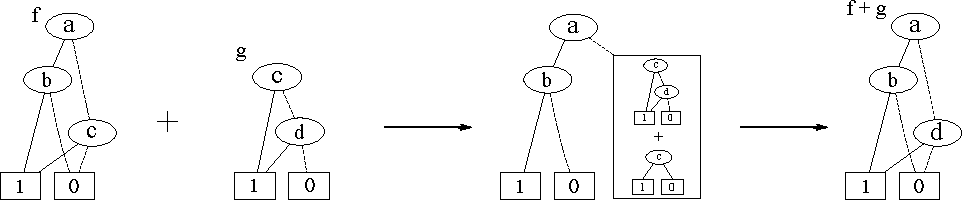
\includegraphics[scale=1]{mod2sumfig_new_1.pdf}
\caption{\textcolor{red}{$f+g\pmod 2$ using ZBDDs}}
\label{mod2sumfig}
\end{figure*}

A similar recursive algorithm is also implemented for $f\cdot g \pmod
2$ operation where the intermediate partial product terms are added
$\pmod{2}$ using the Algorithm \ref{mod2sum}. {\it E.g.,} $f = ab, g =
a+b, f\cdot g = ab + ab = 0$. 


\subsection{GBR $z_i\xrightarrow{G}_+r_i$ under RTTO on ZBDDs}


% The variable ordering imposed on the ZBDDs is the same as the one
% derived through RTTO. Then every path from the root to terminal {\bf
%   1} represents a monomial, with the 1-edge or solid-edge (resp. 0-edge or dotted-edge) denoting
% the presence (resp. absence) of the variable in the
% monomial. Traversing only the solid edges from the root node of a ZBDD to
% terminal {\bf 1} delivers the leading monomial $lm(f)$. The
% child node of the root at the solid edge's end will be referred to as $then$ and the other child as $else$. 

Once the ZBDDs for the circuit have been built and stored in $G$, we
need to perform the canonical \Grobner basis reduction $z_i
\xrightarrow{G}_+r_i$ for each output bit $z_i$. The polynomial $r_i$
will be a canonical representation of $z_i$ in terms of primary
inputs. Reduction $f\xrightarrow{g} r$ requires \textcolor{red}{one} to obtain the leading
monomials $lm(f),lm(g)$ of $f, g$ (Eqn. \ref{eqns:reduce1}).


\subsubsection{Finding the leading monomials under RTTO on ZBDDs}
Recall that RTTO imposes a $lex$ term order on the polynomials using
the variable order $x_1>\dots>x_n$. Moreover, the same variable order
$x_1>\dots>x_n$ is imposed on the ZBDDs. Traversing the
then-edges from the root node of a ZBDD to the terminal {\bf 1}
delivers the leading monomial of that polynomial under RTTO.



\subsubsection{Classical reduction with ZBDDs: Cancel one monomial in
  every step} 

The algorithm for conventional reduction procedure using ZBDDs is
shown in Algorithm~\ref{singlemon}. The input parameters are the ZBDD
of the output bit $z_i$ of the circuit and $poly\_list$ -- a list
containing the ZBDDs for the set of polynomials $F =
\{f_1,\dots,f_s\}$ corresponding to the
gates of the circuit. The algorithm is based on the same principles as
the classical division procedure (Algorithm~\ref{algo:mv_reduce}). 
%The variables in the ZBDD manager are
%declared in the same order as the RTTO. For our example of
%Figure~\ref{ChainOrGate}, the first variable declared in the ZBDD
%manager is $z$, then $f$, and so on. 



%\vspace{-0.2in}

%\vspace{-0.2in}
\begin{algorithm}
\caption{Reduction: Cancel 1 monomial every iteration}
\label{singlemon}
\begin{algorithmic}[1]
{\small
\Procedure{$single\_mon\_red$}{$z_i,poly\_list$}
\For{each $g \in poly\_list$}
\State $lead\_g = leading\_term(g)$
\State $lead\_z_i = leading\_term(z_i)$
\State $quotient = ZBDD\_Divide(lead\_z_i,lead\_g)$
\While{$quotient \neq zero$}
\State $prod = quotient \cdot g$
\State $z_i = z_i + prod$
\State $lead\_z_i = leading\_term(z_i)$
\State $quotient = ZBDD\_Divide(lead\_z_i,lead\_g)$
\EndWhile
\EndFor
\State \Return $z_i$
\EndProcedure
}
\end{algorithmic}
\end{algorithm}

The procedure $leading\_term(g)$ returns the leading term of 
the ZBDD representation of polynomial $g$. 
%The procedure starts at the root node and follows the THEN path until
%it reaches the terminal node 1. The cube of the variables, whose
%corresponding nodes are encountered on this path, gives us the
%leading term of the polynomial. 
If $g$ divides $f$, then the procedure $ZBDD\_Divide(f,g)$ (performs cube division) returns the quotient of the
division,  else it returns zero. Line 8 iteratively computes $z_i = z_i +
{lt(z_i) \over lt(g)}\cdot g$. The polynomial $z_i$ is completely reduced
$w.r.t.$ the polynomial $g$ in the while loop. 
% The $\cdot$ operator
% computes the product of two ZBDDs and the + operator is a modulo 2
% sum: $f + g = f \cup g - f \cap g$. 

\subsubsection{Improved Reduction: Cancel multiple monomials in 1 step}
Next, we will show how $z_i$ can be reduced by a polynomial $g$ {in one step}. In the 
example of Figs. \ref{ChainOrGate} and \ref{red_steps}, the primary output
$z$ is reduced by $f_1$ to get $r_1$. The next  step  
is to reduce $r_1$ by $f_2$ to get $r_2$. To demonstrate our
approach we will show how the reduction of $r_1$ by $f_2$ can be
achieved in one step. There are two monomials in $r_1$ that contain
$y$, namely $yd,y$. Both can be canceled by $lt(f_2) = y$ in one step,
eliminating the need of the while loop in Algorithm~\ref{singlemon}.    

The polynomial $r_1 = yd + y + d$ can be written as $y\cdot(d+1) +
d$. If we perform 1-step reduction of $r_1$ by $f_2$ we get 
the {\it quotient} $d+1$. This quotient is visible as the polynomial
represented by the $then$-node of $r_1$ (Fig. \ref{f2}). So the
reduction can be performed by multiplying $d + 1$ with $f_2$ and
subtracting (adding) this  product to $r_1$ $\pmod{2}$.
% \vspace{-0.1in}
%{\small
\begin{align}
& r_1\xrightarrow{f_2}_+ r_2\\
&= (yd + y + d) + (d + 1)\cdot(y + xc + x + c) \pmod{2}\\
&= 2\cdot(yd + y) + d + (d+1)\cdot(xc + x + c) \pmod{2}\label{eqn:cancelmon}\\
&= \underbrace{d}_{else(r_1)} + \underbrace{(d+1)}_{then(r_1)}\cdot\underbrace{(xc + x + c)}_{else(f_2)}  \pmod{2}
\label{eqn:subexp}
\end{align}
%\vspace{-0.1in}
%Use the follwing notation
%\begin{align*}
%& \text{$head(R_1)$ = 1-branch (THEN) of top-most node of $R_1$} = d + 1,\\
%& \text{$tail(R_1)$ = 0-branch (ELSE) of top-most node of $R_1$} = d,\\
%& \text{$head(P)$ = 1-branch of top-most node of $P$} = f,\\
%& \text{$tail(P)$ = 0-branch of top-most node of $P$} = ec + e + c.
%\end{align*}
%}
As shown in Fig. \ref{f2}, $else(r_1)=d, then(r_1)=d+1$ and
$else(f_2)=xc+x+c$. Moreover, $2\cdot(yd + y) = 0
\pmod{2}$. Therefore, in order to reduce number of operations incurred
in the division process, we directly use the last step as a formula
for reduction:   
%\vspace{-0.05in}
%{\small
\begin{align}
\label{eqn:onestep}
r_1 \xrightarrow{f_2}_+ r_2 %&= d + (d+1)\cdot(xc + x + c) \\
&= else(r_1) + then(r_1)\cdot else(f_2)
\end{align}
% }%

\begin{figure}[hbt]
\centering
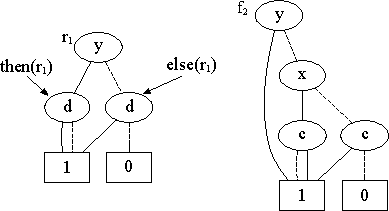
\includegraphics[scale=1]{Preliminaries-Theory/r1_f2.pdf}
\caption{ZBDDs for polynomial $r_1$ and $f_2$.}
\label{f2}
\end{figure}

\textcolor{red}{
%In order for the above equation to be correct in general, 
More generally, to perform the division $r_i \xrightarrow{f_j}_+ r_j$, 
we need to ensure that if $f_j$ divides $r_i$, then the variable
(index) associated with the top-most nodes of  their respective ZBDDs
are the same. This can be ensured by populating
$poly\_list=\{f_1,\dots,f_s\}$ in a certain order.}
%This also results in a significant improvement in
%Algorithm \ref{singlemon} by simplifying the search for the divisors
%$g\in poly\_list$ and is described in the next paragraphs and Example \ref{exm:pi_rtto}.

\textcolor{red}{Due to RTTO, each polynomial $f_j \in F$ is of the form $f_j = x_j +
\text{tail}(f_j)$, where each variable in $\text{tail}(f_j)$
is ordered as being less than $x_j$ (Prop. \ref{prop:top-order}). Due to this order,
the ZBDD representation of the polynomials is of the type $f_1= x_1 +
else(f_1), \dots, f_s= x_s + else(f_s)$, where the variables $x_1,\dots,x_s$ are the 
top-most nodes in their respective ZBDDs with variable order $x_1 >
\cdots > x_s > \cdots > x_n$. Note that the variables
$\{x_{s+1},\dots,x_{n}\}$ are primary inputs, and they are not the output
of any logic gate. {\it We ensure that primary inputs appear last in RTTO.}
Then we store elements in $poly\_list$ according to the order
$f_1 > f_2 > \dots > f_s$; i.e. $poly\_list[1] = f_1,
\dots,poly\_list[s] = f_s$. }

\par \textcolor{red}{Considering Algorithm \ref{singlemon}, suppose
that we first reduce $z_i$ by $poly\_list[1]=f_1$, which results in
variable $x_1$ being replaced by $tail(f_1)$ in $z_i$. The
variable $x_1$ cannot appear  again in $z_i$ at any further reduction
step as $x_1$ is not in the support of  polynomials
$poly\_list[2],\dots,poly\_list[s]$. Further in the reduction process,
let us assume that we have reduced $z_i$ by 
$f_1,f_2,\dots,f_{j-1}$. At this stage the intermediate remainder
$z_i$ will not contain any of the variables $x_1,x_2,\dots,x_{j-1}$ as
they have been canceled by the leading terms of
$f_1,f_2,\dots,f_{j-1}$. The next variable in RTTO is $x_j$.
%
%The variables next to $x_{j-1}$ in RTTO is $x_j$ 
%Therefore, the top-most
%node in the ZBDD of $z_i$ can be any one of the variables
%$x_j,\dots,x_n$. It need to be just $x_j$ as all variables 
%may not be in the logical cone of $z_i$. 
To cancel terms in $z_i$ containing variable $x_j$, we need to search
for the divisor polynomial $f_j = x_j + tail(f_j)$. 
%
There can be two possibilities for $z_i$: 
\begin{enumerate} 
\item If terms in $z_i$ contain
$x_j$, then the top variable of the ZBDD of $z_i$ will be $x_j$. In
  that case, as the top variable of the ZBDD of $f_j$ is also $x_j$,
  $f_j$ can divide $z_i$.
\item If $z_i$ does not contain terms in $x_j$, then the top variable
  of the ZBDD of $z_i$ will not be $x_j$. In that case, $f_j$ (with
  top variable $x_j$) cannot divide $z_i$. 
\end{enumerate}
Therefore, the divisibility of $z_i$ by  the current entry in
$poly\_list[j] = f_j$ can be checked just by comparing the indices of
the top nodes of the ZBDDs of $z_i$ and $f_j$. If the indices 
are equal, then $f_j$ divides $z_i$. Otherwise, $f_j$ does not divide
$z_i$. In terms of the topology of the circuit, the latter case
implies that the gate corresponding to polynomial $f_j$ is not in the
logical cone of $z_i$. 
%
%% If the top
%% variable in the ZBDD of $z_i$ is equal to the top variable in the ZBDD
%% of $f_j$, then $f_j$ divides $z_i$. This search for the divisor $f_j$
%% is equivalent to comparing the indices of top-most nodes of $z_i$ and
%% $f_j$. 
%Otherwise,
%the gate corresponding to the polynomial $f_j$ is not in the logical
%cone of $z_i$.  
%Populating $poly\_list$ in this way avoids the search (Line 4,
%Algorithm~\ref{algo:mv_reduce}) required to find a polynomial $f_j \in
%poly\_list$ that can divide the leading term of $z_i$. 
As a result, imposition of RTTO on the ZBDDs and on $poly\_list$ simplifies the check
for divisors: {\it if indices of top-most nodes of ZBDDs of $z_i$ and
 $f_j$ are equal, then $lm(f_j)$ divides $lm(z_i)$.} 
% \textcolor{red}{The equality of indices indicate that the top variables are the 
% same (as indices are unique). In addition, as $f_i$ is guaranteed to 
% have that variable only in the leading term ($i.e.$ leading term is a singleton 
% with only one variable), $f_i$ divides $z_i$.} 
This allows to 
replace the cube division (Line 5, Algorithm \ref{singlemon}) by an
equality check of top indices of ZBDDs.}

\begin{Example}
\label{exm:pi_rtto}
Consider the step 2 of division corresponding to
 Fig. \ref{ChainOrGate}, where the polynomial $r_1 = yd +y+d$ needs to
 be reduced by $f_2$. RTTO need not differentiate between the
relative ordering of the nets $y, d$ for Prop. \ref{prop:top-order} to
be valid; as both $y, d$ are at the same (reverse) topological
level. However, we ensure that the primary inputs always appear last
in the order. The ZBDDs for $r_1$ and $f_2$ are shown in
Fig. \ref{f2}, where RTTO is lex with $y > x > d > c > b> a$.  As
$index(top\_var(f_2)) = index(top\_var(r_1))$,  $lm(f_2) ~|~ \textcolor{red}{lm(r_1)}$.
If variable $d$ were placed earlier in the order than $y$, then the
top variables of $f_2, r_1$ 
would have been different and we would have had to extract
$lm(r_1),lm(f_2)$ and performed cube division
${lm(r_1)}\over{lm(f_2)}$ to check if $lm(f_2) ~|~ lm(r_1)$. 
\end{Example}


%% While iterating over the polynomials $g \in poly\_list$ if a
%% certain polynomial does not divide the leading term of $z_i$, it 
%%  will imply the polynomial is not in the logical cone of $z_i$.   

Therefore, unlike in Algorithm~\ref{singlemon}, where we need to
obtain the leading monomials and compute the quotient
$lead\_z_i/lead\_g$, now we only need to determine if
$lead\_g$ can divide $z_i$ at all (in which case the quotient is
$then(z_i)$). This can be accomplished by just comparing the indices
of top-most nodes of $z_i$ and $g$. 

\par \textcolor{red}{It can now be shown that Eqn. (\ref{eqn:onestep})
holds throughout the GB-reduction under RTTO. To perform the operation
$r_i\xrightarrow{f_j}_+ r_j$, we consider their ZBDDs constructed
using RTTO. Based on the above discussion, the top variables of the
ZBDDs of $r_i$ and $f_j$ are the same and equal to $x_j$. Also, let $q$
denote the quotient of division of $r_i$ by $f_j$. The operation $r_i
\xrightarrow{f_j}_+ r_j$, is carried out as follows, 
\begin{align*}
r_j &= r_i + q\cdot f_j  
\end{align*}
As $x_j$ is the top variable of $r_i$ and $f_j$, they can be written
as $r_i = x_j\cdot then(r_i) + else(r_i)$ and $f_j = x_j + else(f_j)$,
respectively. Also notice that $q = then(r_i)$, because $f_j$ (with
leading term $x_j$) can only divide the $x_j\cdot then(r_i)$ component
of $r_i$. 
\begin{align*}
r_j &= x_j\cdot then(r_i) + else(r_i) + q\cdot(x_j + else(f_j)) \\
r_j &= x_j\cdot then(r_i) + else(r_i) + then(r_i)\cdot(x_j + else(f_j)) \\
r_j &= 2\cdot x_j\cdot then(r_i) + else(r_i) + then(r_i)\cdot else(f_j) \\
r_j &= else(r_i) + then(r_i)\cdot else(f_j)
\end{align*}} 

\par The last expression is the same as in
Eqn. (\ref{eqn:onestep}). So the reduction process effectively
involves just two operations, a modulo 2 sum and a product. {\it This
  has the effect of canceling all the terms in $r_i$ that can be
  canceled by $lt(f_j)$,  implicitly canceling multiple monomials in
  one step}.  This is made possible only due to the properties that
RTTO imposes on the structure of ZBDDs. 

The algorithm for implicit cancellation of multiple monomials in
GB-reduction is shown in Algorithm~\ref{multimon}, where the notations,
$z_i$ and $poly\_list$, are the same as in Algorithm
\ref{singlemon}. This algorithm significantly
reduces the number of iterations, which now exactly equals the size of
$poly\_list$. For the example of Fig. \ref{ChainOrGate}, the number of
iterations is 3 using Algorithm~\ref{multimon}, whereas 7 iterations
are required using Algorithm \ref{singlemon}.


\begin{algorithm}
\caption{Reduction under RTTO: Cancel multiple monomials}
\label{multimon}
\begin{algorithmic}[1]
{\small
\Procedure{$multi\_mon\_red$}{$z_i,poly\_list$}
\For{each $g \in poly\_list$}
%\State $G_i = POLY\_LIST[i]$
%\State $index_{G_i} = G_i \rightarrow index$
%\State $index_F = F \rightarrow index$

\If{ $index(g) == index(z_i)$} 
%\State $p_1 = then(f)$
%\State $p_2$ = else(f)
%\State tail = else($g_i$)
%\State prod = $p_1$ $ \cdot$  tail
\State $z_i = else(z_i) + then(z_i)\cdot else(g)$
\EndIf

\EndFor
\State \Return $z_i$
\EndProcedure
}
\end{algorithmic}
\end{algorithm}


   

To contrast our approach against PolyBori \cite{polybori:2009}:
PolyBori is a general purpose symbolic computing engine for Boolean
polynomials, whereas our approach (Algorithm
\ref{multimon}) is specific only to RTTO; it would give an incorrect
result of reduction for non-RTTO based term orders. However, our
approach exploits the fact that due to RTTO, the subexpressions
required in the division process are readily
available as the $then$- and $else$-children of the top nodes of the
ZBDD (Eqn. (\ref{eqn:subexp})). Moreover, an implementation using
PolyBori may also generate intermediate monomials that eventually add
up to 0 $\pmod 2$  ($e.g.$ as in Eqn. (\ref{eqn:cancelmon})). Whereas
our approach reduces the size of intermediate computations, and incurs
less computation time, by not generating the duplicate monomials. 


We have implemented the above GBR procedures using the CUDD 
package~\cite{cudd}. The circuit under verification is analyzed, RTTO based
variable order is imposed on the ZBDDs, and the Boolean polynomials of
the circuit are represented as unate cube sets on ZBDDs. 
The polynomials corresponding to the gates of circuit,
$G=\{f_1,\dots,f_s\}$, are inserted in $poly\_list$ according to the
variable order $x_1 > \dots > x_i > \dots > x_n$, where $f_i = x_i +
else(f_i)$. % (this is due to Prop. \ref{prop:top-order}). 
To perform GBR $z_i\xrightarrow{G}_+ r_i$,
Algorithm \ref{multimon} is invoked and $r_i$ used for  equivalence checking. 
%The division algorithm in {\sc
%  polybori} \cite{polybori} is conceptually similar to that of
%Algorithm 1, whereas Algorithm 2 is our main contribution.
